%%%%%%%%%%%%%%%%%%%%%%%%%%%%%%%%%%%%%%%%%%%%%%%%%%%%%%%%%%%%%%%%%%%%%
%% This is a (brief) model paper using the achemso class
%% The document class accepts keyval options, which should include
%% the target journal and optionally the manuscript type.
%%%%%%%%%%%%%%%%%%%%%%%%%%%%%%%%%%%%%%%%%%%%%%%%%%%%%%%%%%%%%%%%%%%%%
\documentclass[journal=jpcbfk,manuscript=article]{achemso}

%\documentclass[english,aps,preprint,pre,floatfix,nofootinbib,showpacs,showkeys]{revtex4-1}
%%%%%%%%%%%%%%%%%%%%%%%%%%%%%%%%%%%%%%%%%%%%%%%%%%%%%%%%%%%%%%%%%%%%%
%% Place any additional packages needed here.  Only include packages
%% which are essential, to avoid problems later. Do NOT use any
%% packages which require e-TeX (for example etoolbox): the e-TeX
%% extensions are not currently available on the ACS conversion
%% servers.
%%%%%%%%%%%%%%%%%%%%%%%%%%%%%%%%%%%%%%%%%%%%%%%%%%%%%%%%%%%%%%%%%%%%%
\usepackage[version=3]{mhchem} % Formula subscripts using \ce{}

\SectionNumbersOn

\usepackage{amsmath}
\usepackage{amssymb}
\usepackage{color}
\usepackage{CJK}
\usepackage{framed}
\usepackage[hidelinks]{hyperref}
\usepackage{algorithm}
\usepackage{algpseudocode}
\algdef{SE}[DOWHILE]{Do}{doWhile}{\algorithmicdo}[1]{\algorithmicwhile\ #1}

\usepackage[scaled=0.85]{beramono}
\usepackage[T1]{fontenc}
\usepackage{changepage}

%%%%%%%%%%%%%%%%%%%%%%%%%%%%%%%%%%%%%%%%%%%%%%%%%%%%%%%%%%%%%%%%%%%%%
%% If issues arise when submitting your manuscript, you may want to
%% un-comment the next line.  This provides information on the
%% version of every file you have used.
%%%%%%%%%%%%%%%%%%%%%%%%%%%%%%%%%%%%%%%%%%%%%%%%%%%%%%%%%%%%%%%%%%%%%
%%\listfiles

%%%%%%%%%%%%%%%%%%%%%%%%%%%%%%%%%%%%%%%%%%%%%%%%%%%%%%%%%%%%%%%%%%%%%
%% Place any additional macros here.  Please use \newcommand* where
%% possible, and avoid layout-changing macros (which are not used
%% when typesetting).
%%%%%%%%%%%%%%%%%%%%%%%%%%%%%%%%%%%%%%%%%%%%%%%%%%%%%%%%%%%%%%%%%%%%%

\makeatletter
    \setlength\@fptop{0\p@}
\makeatother

\newcommand*\mycommand[1]{\texttt{\emph{#1}}}

\newcommand{\state}[1]{$\mathcal{S}_{#1}$}

%\newcommand*{\rood}[1]{\textcolor{red}{#1}}
\newcommand*{\rood}[1]{#1}
%\newcommand*{\blauw}[1]{\textcolor{blue}{#1}}
\newcommand*{\blauw}[1]{#1}
%\newcommand*{\groen}[1]{\textcolor{green}{#1}}
\newcommand*{\groen}[1]{#1}
%\newcommand*{\blauwr}[1]{\textcolor{blue}{#1}}
\newcommand*{\blauwr}[1]{#1}
\newcommand{\Expect}[1]{\mathrm{E}\left[#1\right]}
\newcommand{\norm}[1]{\left\lVert#1\right\rVert}

%\newcommand*{\addref}[1]{\textcolor{red}{\{ADD REF: #1\}}}

\newcommand*{\noter}[1]{\textcolor{red}{[[#1]]}}		% notes on
%\newcommand*{\noter}[1]{}					% notes off

%\usepackage[draft]{todonotes}   % notes shown
\usepackage[disable]{todonotes} % notes hidden
\usepackage{comment}

\usepackage[normalem]{ulem}
\usepackage{algorithm}
\usepackage{subfig}
\usepackage{algpseudocode}

%%%%%%%%%%%%%%%%%%%%%%%%%%%%%%%%%%%%%%%%%%%%%%%%%%%%%%%%%%%%%%%%%%%%%
%% Meta-data block
%% ---------------
%% Each author should be given as a separate \author command.
%%
%% Corresponding authors should have an e-mail given after the author
%% name as an \email command. Phone and fax numbers can be given
%% using \phone and \fax, respectively; this information is optional.
%%
%% The affiliation of authors is given after the authors; each
%% \affiliation command applies to all preceding authors not already
%% assigned an affiliation.
%%
%% The affiliation takes an option argument for the short name.  This
%% will typically be something like "University of Somewhere".
%%
%% The \altaffiliation macro should be used for new address, etc.
%% On the other hand, \alsoaffiliation is used on a per author basis
%% when authors are associated with multiple institutions.
%%%%%%%%%%%%%%%%%%%%%%%%%%%%%%%%%%%%%%%%%%%%%%%%%%%%%%%%%%%%%%%%%%%%%
\author{Michael S. Jones}
\affiliation{%
  Pritzker School of Molecular Engineering, %
  The University of Chicago, %
  929 East 57th Street, Chicago, Illinois 60637, United States%
}

\author{Brennan Ashwood}
\affiliation{%
  Department of Chemistry, Institute for Biophysical Dynamics, and James Franck Institute, %
  The University of Chicago, %
  929 East 57th Street, Chicago, Illinois 60637, United States%
}

\author{Andrei Tokmakoff}
\affiliation{%
  Department of Chemistry, Institute for Biophysical Dynamics, and James Franck Institute, %
  The University of Chicago, %
  929 East 57th Street, Chicago, Illinois 60637, United States%
}

\author{Andrew L. Ferguson}
\email{andrewferguson@uchicago.edu}
\affiliation{%
  Pritzker School of Molecular Engineering, %
  The University of Chicago, %
  929 East 57th Street, Chicago, Illinois 60637, United States%
}

%\author{I. Ken Groupleader}
%\altaffiliation{A shared footnote}
%\email{i.k.groupleader@unknown.uu}
%\phone{+123 (0)123 4445556}
%\fax{+123 (0)123 4445557}
%\affiliation[Unknown University]
%{Department of Chemistry, Unknown University, Unknown Town}
%\alsoaffiliation[Second University]
%{Department of Chemistry, Second University, Nearby Town}

%\author{Susanne K. Laborator}
%\email{s.k.laborator@bigpharma.co}
%\affiliation[BigPharma]
%{Lead Discovery, BigPharma, Big Town, USA}

%\author{Kay T. Finally}
%\affiliation[Unknown University]
%{Department of Chemistry, Unknown University, Unknown Town}
%\alsoaffiliation[Second University]
%{Department of Chemistry, Second University, Nearby Town}

%%%%%%%%%%%%%%%%%%%%%%%%%%%%%%%%%%%%%%%%%%%%%%%%%%%%%%%%%%%%%%%%%%%%%
%% The document title should be given as usual. Some journals require
%% a running title from the author: this should be supplied as an
%% optional argument to \title.
%%%%%%%%%%%%%%%%%%%%%%%%%%%%%%%%%%%%%%%%%%%%%%%%%%%%%%%%%%%%%%%%%%%%%
\title[]{TBA}


%%%%%%%%%%%%%%%%%%%%%%%%%%%%%%%%%%%%%%%%%%%%%%%%%%%%%%%%%%%%%%%%%%%%%
%% Some journals require a list of abbreviations or keywords to be
%% supplied. These should be set up here, and will be printed after
%% the title and author information, if needed.
%%%%%%%%%%%%%%%%%%%%%%%%%%%%%%%%%%%%%%%%%%%%%%%%%%%%%%%%%%%%%%%%%%%%%
%\abbreviations{IR -- infrared, NMR -- nuclear magnetic resonance, UV -- ultraviolet}
%\keywords{Takens}

\begin{document}
%%%%%%%%%%%%%%%%%%%%%%%%%%%%%%%%%%%%%%%%%%%%%%%%%%%%%%%%%%%%%%%%%%%%%
%% The manuscript does not need to include \maketitle, which is
%% executed automatically.  The document should begin with an
%% abstract, if appropriate.  If one is given and should not be, the
%% contents will be gobbled.
%%%%%%%%%%%%%%%%%%%%%%%%%%%%%%%%%%%%%%%%%%%%%%%%%%%%%%%%%%%%%%%%%%%%%

\newpage

\begin{abstract}

\noindent \url{https://www.overleaf.com/project/5e9e5110c524b8000192c548}

\end{abstract}
%%%%%%%%%%%%%%%%%%%%%%%%%%%%%%%%%%%%%%%%%%%%%%%%%%%%%%%%%%%%%%%%%%%%%
%% Start the main part of the manuscript here.
%%%%%%%%%%%%%%%%%%%%%%%%%%%%%%%%%%%%%%%%%%%%%%%%%%%%%%%%%%%%%%%%%%%%%

\newpage

\begin{comment}
%%%%%% intro notes %%%%%%%
\citep{Sanstead2018DirectDehybridization} Good intro with refs and focus on importance of dynamics "rich dynamics even for short oligos" ... Many of the most important functions performed by DNA are highly dynamic, whether in the the biological roles of replication transcription, and gene regulation, or in the expanding field of DNA-based nanotechnology
\end{comment}

\section{\label{sec:intro}Introduction}

Over the last couple decades, DNA has proved to be much more than a vessel for genetic information. From sensing, to computing, to directed self-assembly, the programmable and predictable nature of DNA has unlocked numerous unforeseen applications \citep{Seeman2017DNANanotechnology, Adleman1994MolecularProblems.pdf, Rothemund2006FoldingPatterns, Gu2010ALine}. Recently, structural DNA nanotechnology has enabled self-assembly on micro to milli scales, and dynamic DNA nanotechnology has been used to perform basic calculation and to probe single molecules via temporal DNA signatures\citep{MhatreV.HoJi-AnnLee2012NIHAccess, Bui2018, Shah2019}. Both technologies rely on the hybridization reaction between complementary DNA strands and leverage the flexibility of shorter DNA oligomers to participate in these reactions. Although many experimental and computational studies have rigorously explored DNA dynamical phenomena such as hybridization, hairpin formation, and single base pair flipping, the sequence-dependent mechanisms of hybridization and dissociation dynamics are not fully understood \citep{Yin2011KineticsHybridization, Xiao2019, Hinckley2014Coarse-grainedEffects, Sanstead2016, Porschke1971CooperativeTransition, Porschke1973ThermodynamicsPairs, Chen2007InfluenceHybridization, Craig1971ElaxationOligon}. Moreover, it is unclear the extent to which these processes evolve in an "all-or-nothing" fashion or if an ensemble meta-stable states facilitates the transition. Recent breakthrough studies have coupled experimental techniques with machine learning and MD simulations to investigate and predict sequence-dependent kinetics \citep{Schickinger2018TetheredHelices, Zhang2018PredictingSequence}. Where these studies focus on association and dissociation kinetics alone, we broaden our analysis into higher order dynamical processes and meta-stable intermediates. The stability of certain intermediates states, such as out-of-register or shifted base pairing in repetitive sequences, has been well documented in previous computational studies \citep{Phys2014, Xiao2019, Maciejczyk2014DNAModel}). Furthermore, frayed structures and dynamics have been investigated in numerous computational and experimental studies \citep{Zgarbova2014BaseRNA, Nonin1995TerminalFraying, Nikolova2012ProbingSimulations, Andreatta2006UltrafastHelix}. Sandstead et al. highlighted the role of these dynamics during duplex dissociation, where the stability of frayed states was dictated by G:C base placement 10-mer oligonucleotide sequences \citep{Sanstead2016}. In this work, we study the same four sequences explored by Sandstead et al in an effort to uncover the sequence-dependent dynamics and their relation to metastable structures mentioned above.

Our understanding of DNA dynamics has been built from decades of experiments -- such as temperature-jump, salt-jump, pH-jump, or other perturbative methods -- that drive DNA out of equilibrium and monitor relaxation processes in one direction \citep{Morrison1993SensitiveSolution, Wetmur1968KineticsDNA, Craig1971ElaxationOligon, Porschke1973ThermodynamicsPairs, Williams1989LaserDGCATGC, Narayanan2012ExploringMixing, Chen2007InfluenceHybridization, Sanstead2018DirectDehybridization}. More recently, single molecule diffusion and tethered multifluorophore assays have facilitated equilibrium analysis, however these present technical difficulties and are hampered by data collection rates \citep{Liu20173DSolution,  Schickinger2018TetheredHelices, Chen2008Base-by-baseSpectroscopy, Dupuis2013Single-moleculeHelices}. Förster resonance energy transfer (FRET) analysis, particularly when coupled with methods mentioned above, provides additional resolution, but it is unclear how fluorescent tags may interfere with the dynamics of short nucleotides \citep{Morrison1993SensitiveSolution}. Given that dynamic insights from these experiments are limited, several high-level computational models have been employed to gain further detail \citep{Romano2013DNADependence, Hinckley2013AnHybridization, Maciejczyk2014DNAModel, Markegard2015}. Although these models provide experimentally verified speed-ups compared to all atom simulations, the long timescales on which DNA hybridization and dissociation events occur make these processes difficult to sample via direct simulation techniques \citep{Phys2014}. Instead, many previous studies of DNA hybridization have employed accelerated sampling methods such as umbrella sampling,  transition path sampling, and forward flux sampling \citep{Schmitt2013ExploringSurface, Sambriski2009,  Hoefert2011MolecularOligonucleotides, Romano2013DNADependence}.Other computational works use dramatically elevated temperature or denaturing solvent concentrations induce one-way dissociation events \citep{Wong2008TheSimulations, Perez2010Real-timeUnfolding}. Taken together, most experimental and computational work have studied certain aspect the overall dynamics process in one direction.

\textcolor{purple}{Could add more here about all-atom simulations?} 

In this work, we use the coarse-grain 3 Sites Per Nucleotide (3spn2) model to simulate hybridization and dissociation behavior near each sequence's melting temperature \citep{Hinckley2013AnHybridization}.  We leverage the properties of Markov State Models (MSMs) -- namely that conditional probability depends only on the current state of the system \citep{Pande2010EverythingAsk} -- to combine many independent and unbiased trajectories and develop an understanding of sequence-specific kinetics and thermodynamics. MSMs have recently been implemented to study mechanisms and microstate distributions of DNA hybridization  \citep{Jin2019, Xiao2019}, but the slowest sequence-dependent kinetics were not the focus of these studies. \citet{Pinamonti2017} used MSMs to compare the slowest dynamics of short RNA nucleotides and found that stacking timescales are highly sequence dependent \citep{Pinamonti2017}. We take a similar approach to study 10-mer DNA oligonucleotides and introduce State Free Reversible Vampnets (SRVs) to directly learn the slowest sequence-dependent dynamical modes \citep{Chen}. Furthermore, we integrate SRVs into the MSM pipeline by generating an optimized low dimensional basis in which microstates clustering can be performed. We show that SRV coordinates can be useful for both directly interpreting dynamical trends and for improving overall SRV-MSM quality when compared to more conventional methods such as time-structure independent components analysis (tICA).

We find that GC base pair placement in decamer oligonucleotides has a substantial effect on dynamical behavior. By evaluating equilibrium trajectories we can study the relevance of meta-stable states during both the hybridization and dissociation process. Furthermore we can perform these analyses without biasing simulations or assuming that one processes is a strictly reversible version of the another. Because SRVs generate an optimized low dimensional basis, we show that we can access higher resolution MSMs (shorter lag time) and generate more detailed models. Additionally, we can compare slow dynamical modes and meta-stable states between sequence-specific SRV-MSMs. Within these meta-stable dynamical states, we leverage diffusion maps to analyze the diversity of structures whose inter-conversion rate are too fast to produce unique slow modes. Finally, we run higher temperatures simulations to investigate the temperature-dependent nature of some experimentally relevant DNA dynamics \textcolor{purple}{Not sure how much to say about this here, but I think these experiments should be mentioned in the intro}. Taken together, our analysis reflects similar results to previous computational and experimental DNA work, while elucidating new insights into sequences dependent dynamics, meta-stable structures, and relative timescales. 

\section{\label{sec:methods}Methods}

\subsection{\label{sec:methods}3spn2 Model}

\textcolor{purple}{Is some additional information warranted on the model itself before going into this specific setup?}

\subsection{\label{sec:methods}Simulation set up}

We initialized four sequences previously investigated by Sandstead et al. -- 5'ATATATATAT3' (AT-all), 5'GATATATATC3' (GC-end), 5'ATATGCATAT3' (GC-core), and 5'ATGATATCAT3' (GC-mix) -- along with their complementary strands according to 3SPN.2 documentation \citep{Sanstead2016, Phys2014}. We initialized explicit ions such that 240 mM NaCl and 18 mM MgCl2 were added to the box in addition to 18 Na counter ions to balance the charge from the 9 phosphate groups in each oligonucleotide backbone \citep{Hinckley2015}. In order to maximize concentration without allowing strands to see each other through periodic boundaries, we set the box size just larger than the sum of the maximum end-to-end extension length of a single strand and the force cutoff (using Ewald summation method is set at 20 A). This translated to a box size of 77.74 Å and an effective oligo concentration of 7 mM. We used an Ewald potential to calculate long range Coulombic interaction between DNA and ions. We used a Debye-Huckel screening potential to account for phosphate-backbone interactions and preserve the persistence length and intrinsic curvature of DNA while taking the effects of ion-DNA interactions\citep{Hinckley2015}. We ran our simulations in the NVT ensemble and fix temperature via a Langevin thermostat in order to model implicit solvent interactions \citep{Schneider1978Molecular-dynamicsTransitions}. We set the simulation temperature was set about 1 K higher than empirical sequence-specific melting temperature in order to maximize transitions between dissociated and hybridized states. We use a 15 fs time step and $3*10^{8}$ steps in each simulation, equating to 4.5$\mu$s simulation time. Base pair coordinates were saved every 30 ps, and full frames including backbones and ions were saved every 3 ns for visualization purposes. For each sequences, 100 simulations were performed in parallel, consuming about 32 serial cpu-hours of computation time for each independent simulation. An approximate Tmelt Boltzman distribution was replicated by initializing half of runs from the hybridized state and half from a random dissociated state. In order to allow for further equilibration, the first third (1.5 $\mu$s) of each simulation was removed, resulting in 100 x 100000 frames and a total of 300$\mu$s simulation time per sequence.

\subsection{\label{sec:methods}Featurization}

All intermolecular pairwise distances for both oligonucleotides were calculated at each frame using the MDtraj software package \citep{McGibbon2015MDTraj:Trajectories}. Based on the self-complementary nature of each sequence, we averaged permutable distances (45 pairs in total) together. This permutation reduction follows a similar procedure used in TICAgg coordinates construction \citep{Sengupta2019AutomatedSelf-assembly}. The VAMP-2 scoring method was employed to evaluate the kinetic variance of the feature set and optimize hyperparameters \citep{WuVariationalData, Mardt2018VAMPnetsKinetics}. The VAMP-2 score uses the covariances of a set of inputs estimates the transfer operator of a dynamical system (equation below), providing a robust and object means to evaluate various parameters and models. In the equations below, we show how covariances are obtained from some featurization $\chi$ of a time series $x_t$ and its time-lagged pairs $x_{t+\tau}$. The score $R_2$ can then be found for $\chi$ by applying the VAMP principle with cross-validation.

\begin{align}
 	\mathscr{C}_{00}=&\Expect{\chi(x_t)\chi(x_t)^\intercal}_t\\
 	\mathscr{C}_{01}=&\Expect{\chi(x_t)\chi(x_{t+\tau})^\intercal}_t\\
 	\mathscr{C}_{11}=&\Expect{\chi(x_{t+\tau})\chi(x_{t+\tau})^\intercal}_{t+\tau}\\
	\\
 	R_2[\chi]=&\norm{\mathscr{C}_{00}^{-1/2}\mathscr{C}_{01}\mathscr{C}_{11}^{-1/2}}_F^2 +1
 	%R_2^{val}[\chi]=&\norm{\mathscr{(C_{00}^{val})}^{-1/2}\mathscr{C}_{01}^{val}\mathscr({C}_{11}^{val})^{-1/2}}_F^2 + 1
\end{align}\label{CK1}

% for more general case with  \chi_0, \chi_1, but in practice this is not used
\begin{comment} 
\begin{align}
 	\mathscr{C}_{00}=&\Expect{\chi_0(x_t)\chi_0(x_t)^\intercal}_t\\
 	\mathscr{C}_{01}=&\Expect{\chi_0(x_t)\chi_1(x_{t+\tau})^\intercal}_t\\
 	\mathscr{C}_{11}=&\Expect{\chi_1(x_{t+\tau})\chi_1(x_{t+\tau})^\intercal}_{t+\tau}\\
	\\
 	R_2[\chi_0, \chi_1]=&\norm{\mathscr{C}_{00}^{-1/2}\mathscr{C}_{01}\mathscr{C}_{11}^{-1/2}}_F^2\\
 	R_2^{val}[\chi_0, \chi_1]=&\norm{\mathscr{(C_{00}^{val})}^{-1/2}\mathscr{C}_{01}^{val}\mathscr({C}_{11}^{val})^{-1/2}}_F^2 + 1\\
\end{align}\label{CK2}
\end{comment}

We compared scores for the permutation-free distances, intermolecular, and intra+intermolecular distances and found small differences between the three that varied by sequences (show all sequences in supplemental), but overall we did not observe a loss in kinetic information when using the reduced feature set. We found a substantial increase in VAMP-2 score when using reciprocal pairwise distances and chose reciprocal permutation-free coordinates as a consistent feature set. These features were normalized and passed into sequence-specific SRVs. 

% include covariance, vamp-2  and validation equations, lag time equation from vampnet paper mardt2018

\subsubsection{\label{sec:methods}SRVs}
 
SRVs were first developed by Chen et al. as a means to directly learn slow eigenfunctions of the transfer operator \citep{Chen}. The framework uses a twin-lobed artificial neural network, similar in structure to the network employed in VAMPnets \citep{Mardt2018VAMPnetsKinetics}, to learn a low dimensional representation of input features. This representation is optimized for the variational approach to conformational dynamics (VAC) from which the leading eigenfunctions of the transfer operator are then estimated. The resulting orthogonal modes are associated with the slowest dynamical processes in a system, and can be used to interpret kinetic information directly (such as physical correlations and timescales) and to construct MSMs. Other methods, such as time-lagged independent component analysis (TICA) and kernel TICA (kTICA), have been employed in place of SRVs but suffer limitations from the linear transformation in the case of the former and high computational cost in the case of the latter \citep{Molgedey1994SeparationCorrelations, Harrigan2017LandmarkDynamics}. SRVs provide robust nonlinear approximation and computation time that scales linearly with the amount of input data. This is a key attribute to our system as 10 million frames with 55 features in each frame are used as input data. The SRV framework has been tested on toy systems where the true eigenfunctions of the transfer operator are known and on small protein simulation data such as the WW-domain and Trp-cage mini-protein \citep{Chen, Sidky}. For these latter system, SRV-MSMs were contructed in order to find the stability of metastables states as well as transition probabilities between those states.

Using optimized hyperparameters and featurized trajectory data, we transform 55 reciprocal pairwise distances into a low dimensional SRV basis set. In order to maintain consistency between sequences, we kept all SRV training hyperparameters the same with the exception of the number of outputed slow modes. We determined the number of slow modes via cross-validation on the VAMP-2 score to ensure that the coordinate did not over fit on statistical noise \citep{McGibbon2015VariationalKinetics}. In particular, we looked for convergence in the vamp-2 score and inconsistency between cross validation scores -- suggesting that the model may be overfitting on artifacts in the training data. We used a batch size of 50000 and ran each model for a total of 30 training epochs. We used two hidden layers and set the size of each layer to 100. For cross-validation and comparison between different hyper-parameters, we used a 80/20 validation split training. SRV training required about 22 GPU-minutes across 1 GPU and 10 CPUs. SRV training was implemented using Keras and Tensorflow \citep{KerasGithub.Com, Abadi2016TensorFlow:Systems}.

\subsubsection{\label{sec:methods}SRV-MSMs}

MSMs are a powerful tool for interpreting large amounts of simulation data in a statistically robust and experimentally comparable way. The technique relies on the discretitization of kinetically similar conformations into microstates and finds the conditional probability between states within some lag time. The reliance on conditional probabilities allows for many independent simulations (longer than the lag time) to be collectively interpreted. To take full advantage of the MSM frameworks, however, the input basis should be as kinetically meaningful as possible \citep{Pande2010EverythingAsk}. This becomes crucial in our system given the large difference in timescales between leading modes. Because SRV eigenfunctions translate simulation features into their slowest kinetic representations, they are optimally suited as an MSM basis. To prove this, SRV-MSM VAMP-2 scores were shown to be consistently higher than MSMs constructed from TICA coorinates (TICA-MSMs) \citep{Sidky}. Furthermore, SRV-MSM implied timescales converge faster than TICA-MSM timescales, enabling a shorter lag time and therefore a higher resolution model. To build our SRV-MSM framework, we employed the PyEmma MSM pipeline and generated independent models for each sequence \citep{Scherer2015PyEMMAModels}. After passing in SRV coordinates, we perform k-means microstate clustering, Bayesian MSM construction, and PCCA+ hierarchical macrostate assignments. The number of microstates were determined by VAMP-2 score, and the SRV-MSM lag time was selected based on implied timescales convergence.  The number of PCCA+ macrostates was determined based on the characteristic of each system and will be discussed more in depth in the results. 

%%%%%%%%%%%%%%%%%%%%%%%%%%%%%%%%%%%%%%%%%%%%%%%%%%%%%%%%%%%%%%%%

\section{\label{sec:Results}Results}

\subsection{\label{sec:Results}AT-all}

\subsubsection{\label{sec:Results}SRV optimization and analysis}

In our analysis, we found that the AT-all sequence, given its repetitive structure and lack of GC-content, produced the cleanest dynamics and displayed a canonical spectral gap between modes. For this reason, we lead our discussion with this sequence and use it as a case study to work through our SRV-MSM pipeline step-by-step. Our first task was to identify the SRV lag time that was longer than the intrinsic Markov timescales of the system, yet short enough to resolve the dynamics of interest \citep{Phys2018MarkovValidation}. We found that most implied timescales converge at an SRV lag time of 600 ps. We kept a looser constraint on the convergence of the leading mode -- corresponding to the overall hybridization/dissociation process -- as it tends to have a longer transit period and becomes more difficult to fulfill Markovian conditions. It should be noted that our lag time selection was informed by the other sequences as well to maintain consistency. Next we selected an optimal number of SRV components to include in our analysis. After a certain point, higher order dynamical modes provide diminishing contributions the overall kinetic variance as measured by the Vamp-2 score, and the model can begin fitting on statistical noise in the trajectory data instead of the true dynamics \citep{McGibbon2015VariationalKinetics}. It is also more difficult to perform kmeans clustering on a high dimensional space, especially when those higher dimensions are less kinetically relevant \citep{Pande2010EverythingAsk}. For these reasons, the number of slow SRV components should be carefully selected based on the specific system of interest. As shown in (Figure \ref{fig:srv_crossval-AT-all}), we see diminishing returns in the VAMP-2 score after five slow modes and select these modes as our optimized SRV basis. Next, we seek to interpret the physical relevance of these leading modes by plotting the Pearson correlation of each mode with the 100 intermolecular distances between strands. The quantitative meaning of these coordinates can be difficult to interpret given their nonlinear relationship to the SRV collective variables, but the relative different between these correlations shows which coordinates are most affected by (or effective on) each process. For example, the first slow mode shows a significant positive correlation to each distance and the strongest correlation with matching base pair distances (shown along the main diagonal). Given these relationships and the substantially longer timescale of this process, we can deduce that this leading mode corresponds to the dynamics of the overall hybridization and dissociation process. The next four SRV components all show a relatively high correlation along different offset diagonals. These diagonals correspond to the intermolecular distances between shifted base pairs and point to the existence of gradually faster shifting or "slithering" processes. Slow slithering mechanisms have similarly been reported in simulation studies to occur on orders of magnitude longer timescales than underlying fast dynamics such as fraying \citep{Markegard2015, Xiao2019, Maciejczyk2014DNAModel}.

\begin{figure}[ht!]
	\begin{center}
        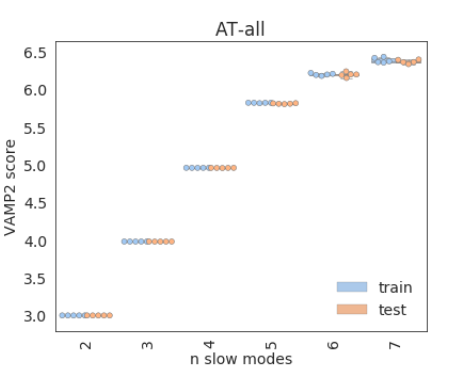
\includegraphics[width=50mm, 
        scale=0.5]{Figs/figs_0804/srv_crossval-AT-all.png}
        \caption{5-fold cross validation procedure to select number of SRV coordinates. We look for both the converge of the VAMP-2 and consistent scores between folds to ensure that the model is not fitting on statistical noise. For AT-all we observed a spectral gap after the 5th coordinate. Cross-validation on other sequences is in the SI. (Add AT-all feature scores here as well?)}
        \label{fig:srv_crossval-AT-all}
	\end{center}
\end{figure}

\subsubsection{\label{sec:Results}SRV-MSM construction and optimization}

From this analysis we can determine that the slowest dynamics are fully characterized by the hybridization process and slithering behavior of out of register base pairs. Although this is qualitatively informative, we can access a more holistic picture of sequence kinetics and thermodynamics by using these SRV coordinates as a basis on which to construct an MSM. Because these coordinates are already capturing a majority of the system's kinetic variance, they serve as an ideal basis on which to group frames into microstates. We performed k-means clustering, and optimized the number of microstates at 200 by monitoring VAMP-2 score. Next, we selected an MSM lag time in a similar fashion to our SRV lag time selection process. In Figure \ref{fig:AT-all_dynamic} we compare the convergence of SRV-MSM and TICA-MSM timescales, where SRV-MSM timescales converge consistently faster and to higher values of all leading modes. This enables us to select a shorter lag time and build a higher resolution model than we could from an analogous TICA basis. Using an MSM lag time of 1.2 ns, we then built a Bayesian MSM to calculate transition probability matrix between each microstate. Finally, PCCA+ spectral clustering was implemented to group these microstates into macrostates that each represent a collection of metastable structures. Previous work have used a common set of microstates and/or performed manual clustering of microstates based on physical read outs from simulation data (stacking score, energies, etc) \citep{Pinamonti2017PredictingModels, PinamontiTheModels}. Although these techniques are useful for performing comparisons between sequences, we saw better results when optimizing MSMs to capture the most detail of sequence individually and thus developed an independent set of microstates and macrostates for each sequence. For AT-all, we kept to the convention of clustering into n+1 macrostates, where n is the number of slow components captured by the MSMs. To visualize these six macrostates, we project the data into the two leading TICA coordinates. Although SRVs outperform these coordinates for the purpose of MSM construction, TICA represent good high variance collective variables on which to visualize free energies and state assignments \citep{Sidky}. It is clear in Figure \ref{fig:AT-all_in_one} that the PCCA state assignments are capturing free energy minima in TICA space as independent states. After assigning these macrostates we can then calculate their relative probabilities and free energies, visualize representative molecular renderings, and estimates transition probabilities between states. In this final step, we use a minimum flux cutoff of 2e-6 in order to mitigate erroneous quick transition or skipping between states. 

\begin{figure}[ht!]
	\begin{center}
        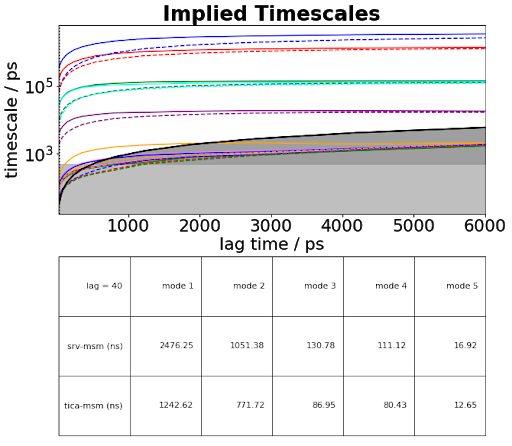
\includegraphics[width=\textwidth]{Figs/figs_0804/AT-all_dynamic.png}
        \caption{AT-all SRV-MSM timescales convergence and implied timescales using a lag time of 1.2 ns. Leading slow mode correlations to all 100 intermolecular distances between oligos.}
        \label{fig:AT-all_dynamic}
	\end{center}
\end{figure}

\subsubsection{\label{sec:Results}Implied timescales for TICA-MSMs for }

In our coarse-grained SRV-MSM, we observe an "aligned hybridized" state, dissociated state, and four "shifted" states characterized by different combinations of out-of-register base pairings. These shifted states consist of 2 or 4 base pair shifting (single or doubled shifted) in either the 5' or 3' direction with varied stability and transition fluxes between kinetically neighboring states. This state decomposition is expected given the repetitive nature of the AT-all sequence and previous computational results that find shifted conformations form "deep kinetic traps" \citep{Xiao2019, Phys2014}. We found a substantial difference in thermodynamic stability and kinetic behavior between the 5'A shifted states and 3'T shifted states. This difference can be accounted for by examining experimental studies on the thermodynamics of "dangling ends" -- unpaired bases adjacent to the paired duplex -- and "inert tails" -- free bases that extend beyond the dangling end \citep{Michele2014EHybridization}. Dangling 5' ends have a consistently stabilizing effect, and inert tails tend to decrease stability as they increase in length, particularly at lower ionic strengths. It has been shown that 5' dangling ends with one inert tail have higher melting temperatures and are energetically favorable compared to 3' ends \citep{Senior1988InfluenceDuplexes, Dickman2012ThermodynamicDNAs}. This is likely due to 5' ends preferentially stacking on the core duplex compared to 3' ends and/or 3' ends binding few counterions and perturbing the duplex structure and solvation environment \citep{Doktycz1990ThermodynamicATGC}. Furthermore, DNA nearest neighbor (NN) calculations that include dangling end contributions (Figure \ref{fig:AT-all_in_one}) predict that the specific nearest neighbors bonds in the 5' shifted state are more energetically favorable than those in the 3' shifted state. Although NN calculations were accurate in predicting the intact thermodynamics behavior of these sequences, they assume all-or-nothing hybridization and do not take inert tails into account \citep{Santalucia2004TM, SantaLucia1998AThermodynamics} Taken together, these experimental results substantiate why we observe the single-shifted 5' state to be only slightly less stable relative to the aligned hybridized state. Furthermore, we expect implied timescales of the two leading modes to be on the same order of magnitude as these reflect the average "dwell" time between transition into and out of these states. The stability of the single-shifted 3' state is notably lower than that of the single-shifted 5' state. In fact, the free energy is about equal to that of the double-shifted 5' state, despite it having two less intact base pairs. This is partially explained by nearest neighbor calculations, however these do not account for the differential effects of the 5' and 3' inert tails or kinetic considerations which we will discuss more below. The double-shifted 3' state is more stable than one might expect given the difference in stability between the single and double 5' shifted states. This might be attributed to the asymptotic effects of inert tail destabilization -- longer tails tend to have a diminishing effect on overall strand stability \citep{Michele2014EHybridization}. Accordingly, the longer inert tails in the double-shifted states have less of an effect on relative 5' vs. 3' stability compared to the shorter tails in the single-shifted states.

\begin{figure}[ht!]
	\begin{center}
        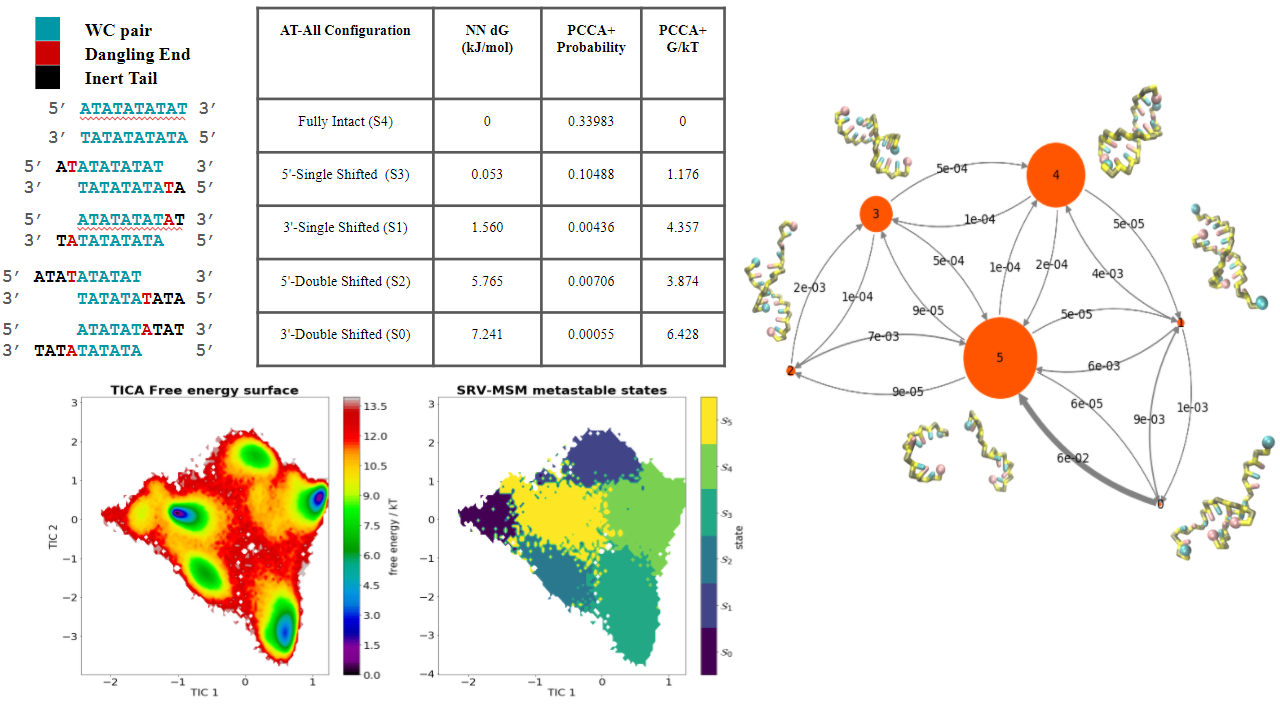
\includegraphics[width=\textwidth]{Figs/figs_0804/AT-all_in_one.PNG}
        \caption{a) Thermo value calculated from Santalucia data and from MSMs b) TICA projections of freen energies and state clustering c) and transitions probabilities between states}
        \label{fig:AT-all_in_one}
	\end{center}
\end{figure}

\subsubsection{\label{sec:Results}Transition probabilities between states}

Beyond state probabilities and free energy approximations, the macrostate MSM yields valuable discrete kinetic information in the form of transition probabilities between states. Figure \ref{fig:AT-all_in_one} shows the probability of moving from one state to another within the MSM lag time (1.2 ns). All transition probabilities are higher when moving towards a more aligned state than towards a more shifted state, suggesting that these metastable shifted states play a more significant role in facilitating the hybridization process than dissociation. Furthermore, we see equal or higher transition rates from shifted states to the dissociated state than to more aligned states, indicating that the slithering-hybridization process is frequently disrupted by complete dissociation. In particular, we observe that the transition probability from double-shifted 3' state to the dissociated state is 6x higher than to the neighboring single-shifted 3' state. Although there is an approximately equal probability of transitioning from the dissociated state to the hybridized and 5' shifted states, there is a 2x lower probability of moving to the 3' shifted states. These asymmetric kinetic effects may have some role in the substantially lower state populations we see above. From these observations we conclude that shifted states are important in facilitating the hybridization process, but that increasingly shifted states (in particular when shifted in the 3' direction) are more likely to dissociate than to evolve into a fully aligned hybridized state. We recognize that these effects could be sensitive to the specific ion environment -- especially considering the effect of ionic strength on inert tails -- and warrant further computational and experimental investigation beyond this work.

For all proceeding sequences, we use the same SRV and MSM lag times, number of microstates, and cross-validation procedures as in the AT-all case. Although these might not represent fully optimized hyperparameters for each sequence, they preserve Markovian properties of the system and provide adequate resolution to evaluate macrostates \textcolor{purple}{not sure if this undermines the point I make earlier about building unique microstates and macrostates for each sequence so as to optimize the model}. The number of SRV coordinates and MSM macrostates are varied based on the kinetics and thermodynamics behavior of specific sequences.

%%%%%%%%%%%%%%%%%%%%%%%%%%%%%%%%%%%%%%%%%%%%%%%%%%%%%%%%%%%%%%%%

\subsection{\label{sec:Results}GC-end}

\subsubsection{\label{sec:Results}SRV-MSM construction and states}
	
Next we examine the GC-end sequence, which add GC caps to the same repetitive AT motifs. Based on SRV cross-validation (SI) we use the leading four slow modes to define our MSM basis.  These coordinates are qualitatively similar to those we studied for AT-all, where the three faster modes each represent some slithering dynamics. When we build the SRV-MSM for the GC-end sequence we observe a larger separation between the leading SRV-MSM timescale and the proceeding modes, which is shown in SI Figure \ref{fig:GC-end_dynamic}) by a distinct spectral gap. We observe a second spectral gap after the fourth slow modes along with a drop in the model vamp-2 score (SI Figure \ref{fig:srv_crossval}). The clustered macrostates show a similar distribution where shifted populations are notably lower. The 3' double-shifted state is no longer identified as a metastable state, and the total number of states is reduced to five (again one more than the total number of slow modes). Although these states appear similar to the AT-all shifted states, the presence of the C:T or G:A mismatches replace two intact WC bonds in the corresponding AT-all states. This substantially diminishes the stability of the GC-end shifted states, resulting in lower state populations and shorter timescales.

\begin{figure}[ht!]
	\begin{center}
        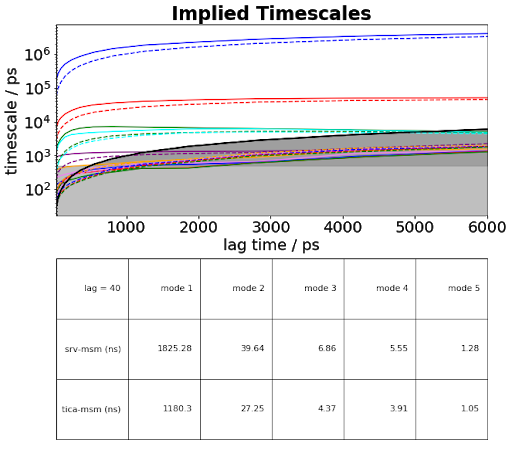
\includegraphics[width=\textwidth]{Figs/figs_0804/GC-end_dynamic.png}
        \caption{(SI) GC-end SRV-MSM timescales convergence and implied timescales using a lag time of 1.2 ns. Leading slow mode correlations to all 100 intermolecular distances between oligos.}
        \label{fig:GC-end_dynamic}
	\end{center}
\end{figure}

\subsubsection{\label{sec:Results}Comparison between GC-end and AT-all shifted states}

For our analysis, we consider C:T and G:A base pairs in the GC-ends shifted states as non-interacting dangling ends such that each shifted conformation has four total dangling ends and two inert tails. Although internal base pair mismatches can cause substantial conformational distortions such as kinking, terminal mismatches have been shown to be slightly stabilizing and have a minimal effect on helical character \citep{Santalucia2004TM, DiMichele2014EffectHybridization}. In the context of the 3spn2 model, these ends are accounted for via intra-strand base stacking and inter-strand cross-stacking interactions \citep{Hinckley2013AnHybridization}. The only direct interaction between non-WC basepairs is parameterized by isotropic excluded volume potential, which is likely much more simplistic than the true mismatch interaction. Despite fewer intact base pairs, we find these structures stabilizing enough to account for the relatively small population of conformations we observed in these shifted states (Figure \ref{fig:GC-end_in_one}). Contrary to AT-all thermodynamics, nearest neighbor calculations predict the 3' shifted states to be slightly more stable than 5' shifted states, again without taking into account entropic or enthalipic (electrostatic) effects from inert tails \textcolor{Purple}{Message here should be that inert tails, looping, other effects have more substantial contribution than two-state NN calculation alone}. However, state populations reveal that the 5' single-shifted is again significantly more stable than the 3'. Interestingly, we found that 5' single-shifted stability might be elevated by a substantial portion of conformations retaining one intact GC base pair. Visualizations reveal that the shifted oligos -- particularly in the 5' shifted state -- have a tendency to sacrifice some helical conformational entropy in a way that facilitates G:C termini bonding even when all available A:T bonds are formed out-of-register.

\begin{figure}[ht!]
	\begin{center}
        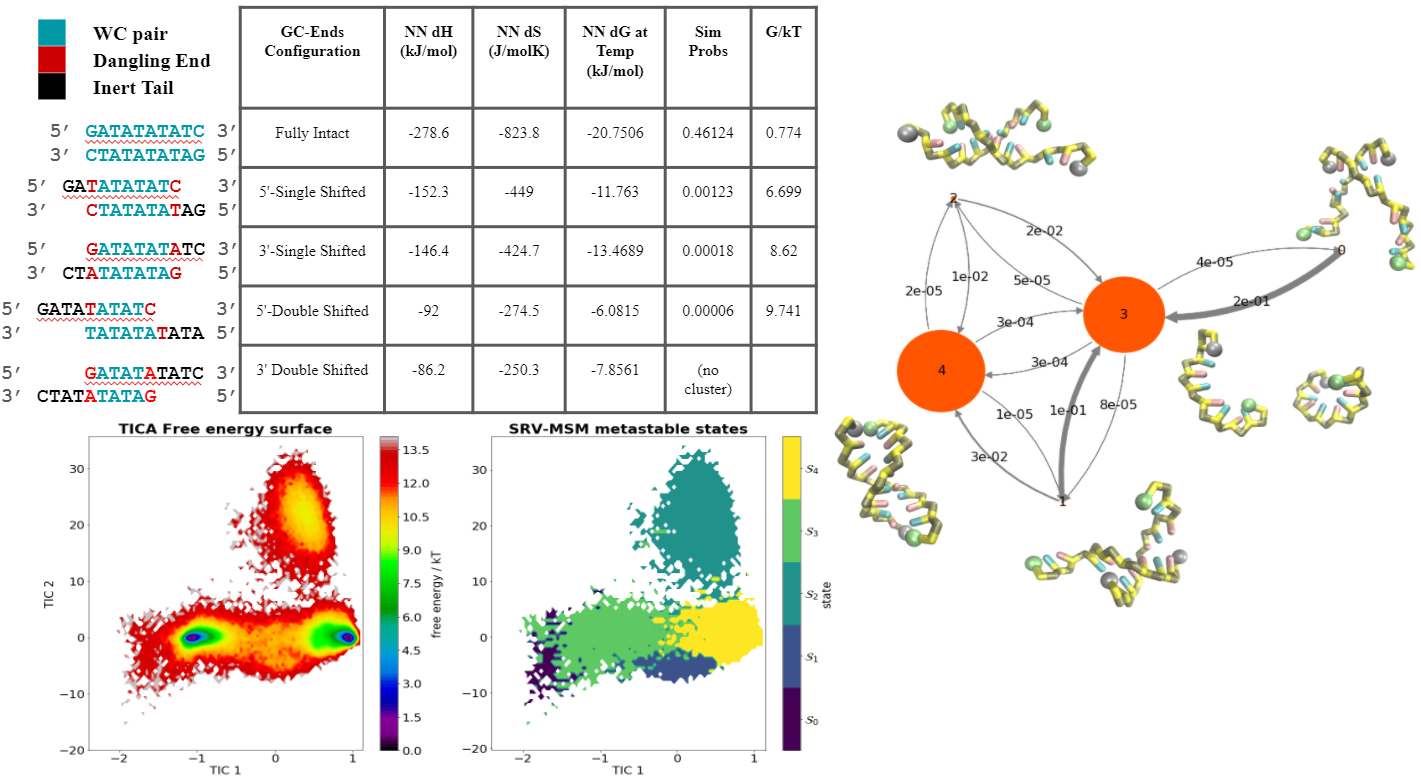
\includegraphics[width=\textwidth]{Figs/figs_0804/GC-end_in_one.PNG}
        \caption{a) Thermo value calculated from Santalucia data and from MSMs b) TICA projections of freen energies and state clustering c) and transitions probabilities between states \textcolor{Purple}{Need to fix 5' double shifted sequence, make same adjustments as for AT-all above}}
        \label{fig:GC-end_in_one}
	\end{center}
\end{figure}

\subsubsection{\label{sec:Results}Diffusion maps show sequence differences in shifted states}

To compare these single-shifted 5' prime states with the corresponding AT-all state, we employ diffusion maps built on an equal sampling of 5000 conformations from 5' shifted state of both sequences. Diffusion maps generate a low dimensional embedding based on some metric for diffusive distance and are well-suited to find subtle structural differences in temporally disconnected data \citep{Coifman2006DiffusionMaps, Ferguson2010SystematicMaps}. We used all 100 intermolecular distances (as opposed to the 55 permutation free coordinates used to construct SRV-MSM) as our distance metric, making it easier to discern structures that form on either identical end of the shifted conformation. This created a degenerate 2nd and 3rd diffusion modes, with nearly equal eigenvalues, differentiating between looping at the identical "top" and "bottom" of the strands. In Figure \ref{fig:GC-end_dmaps} we present the first two non-trivial diffusion map eigenfunctions and show representations of the degenerate third coordinate in the SI (Figure \ref{fig:GC-end_dmaps_full}. Diffusion maps built from samples of the 3' shifted states are also shown in the SI. The first diffusion mode clearly delineates between the GC-end and AT-all shifted conformations and correlates highly with the average distance between the 3' end and its shifted complementary pair. This reveals that the mismatch C:T-pairs are never bound -- a consequence of the excluded volume interaction \textcolor{purple}{state explicitly that C and T have greater excluded volume than G and A in 3spn.2}-- whereas the AT-all pairs are mostly bound with occasional fraying indicated by small AT-all overlap in the GC-end region. This effect may be exaggerated given that C and T base pairs are assigning slightly higher exluded volume radii in 3spn2. The second diffusion mode, which correlates highly with the average distance between 3' and 5' ends, has higher values for GC-end than AT-all. Because the GC-end termini do not bind out of register, we find that they are readily able to form stabilizing contacts despite the shifted conformation of the duplex as a whole. These "shifted-loop" bonds are shown to be uniquely stable for GC-end conformations in the 5' shifted state, and their existence in the simulations confirmed by molecular renderings of these regions Although AT-all shifted ends tend to stay bound out-of-register, the second diffusion coordinate shows some population of inert tails that fold back onto the helix.

\begin{figure}[ht!]
	\begin{center}
        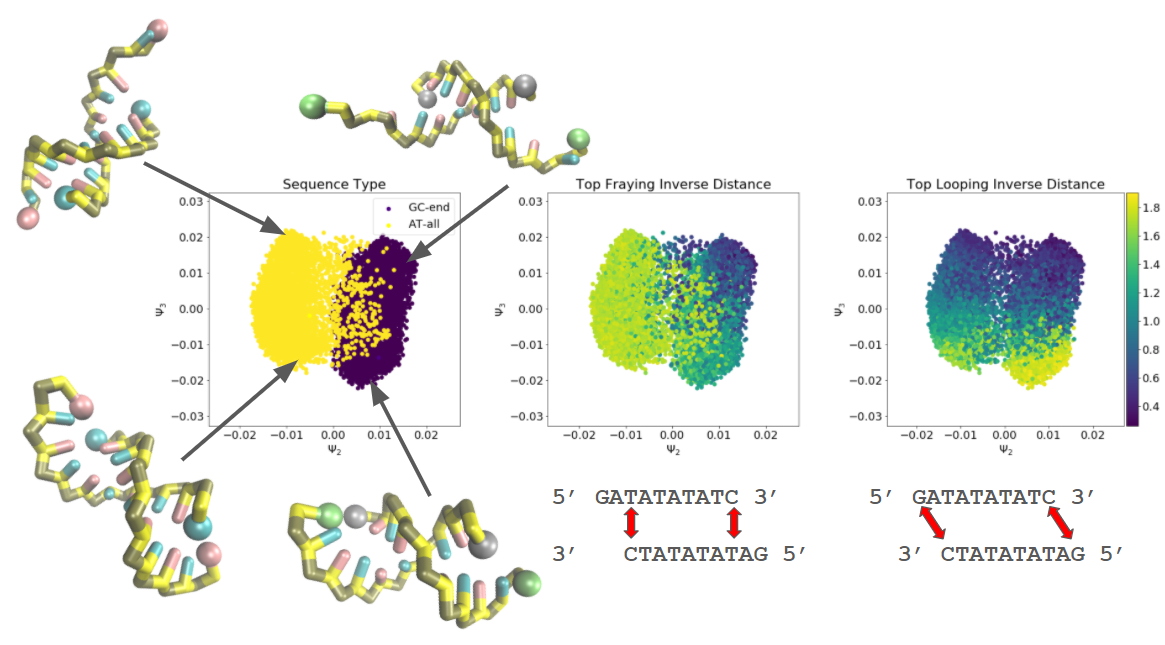
\includegraphics[width=\textwidth]{Figs/figs_0804/GC-end_dmaps.png}
        \caption{First two diffusion map coordinates built from 10000 single-shifted 5' states, equally sampled from AT-all and GC-end. Color maps show inverse distances between out-of-register ends and complementary ends. }
        \label{fig:GC-end_dmaps}
	\end{center}
\end{figure}


\subsubsection{\label{sec:Results}GC-end dynamics are largely two-state}

The kinetic behavior between GC-end macrostates is also distinct compared to AT-all. We do not observe any significant flux between the double-shifted to single-shifted 5' states. While this could be due to insufficient sampling, it is likely that the double-shifted states has too few contacts to directly transition into a single-shifted state without first dissociating. This is further demonstrated by the kinetic distance between this state and the aligned hybridized state (S0 and S4, respectively) shown in TICA projections (Figure \ref{fig:GC-end_in_one}). We observe some flux between the single-shifted states and aligned hybridized state, but these events are more rare than their AT-all equivalents. This suggests that although these transitions are possible routes for hybridization/dissociation, it is substantially more common for the transition to proceed in a two-state manner. In T-jump, FTIR, and 2D IR experiments, the GC-end sequence was observed to have less deviation from the two-state dissociation model compared to oligonucleotides with GC pairs closer to the core \citep{Sanstead2016}. Furthermore, there was a distinct kinetic response -- particularly at lower temperature -- that did not clearly match the fraying processes under investigation. \citep{Sanstead2018DirectDehybridization}. Given that this signal contained some A:T and G:C character and was slower than single base pair fraying, it is possible that it represented some shifted or related looping dynamics. This cannot be verified given that the signal was recorded in a congested spectroscopic range and could be hard to differentiate from aligned G:C fraying. We will discuss this more in our investigation of higher temperatures.


%%%%%%%%%%%%%%%%%%%%%%%%%%%%%%%%%%%%%%%%%%%%%%%%%%%%%%%%%%%%%%%%

\subsection{\label{sec:Results}GC-core}

\subsubsection{\label{sec:Results}Building SRV-MSM}

The GC-core sequence represents a departure from the dominant slithering dynamics observed for AT-all and GC-end. Based on SRV cross-validation (SI Figure \ref{fig:srv_crossval}), we selected the first three components for our analysis. Next, we built an SRV-MSM using these first three SRV modes as a basis and proceeded along the pipeline as described above. We found that four macrostate clustering was unstable -- likely because the 3rd mode is mostly providing  information about dissociation dynamics -- so we performed PCCA+ clustering into three macrostates representing the hybridized, dissociated, and "4bp-frayed" states. Again, we found transition probabilities between states and visualized representative molecular renderings. We observe that the 4bp-frayed meta-stable state is solely composed of trajectories where both G:C core base pairs are bound and one of the adjacent A:T bonds are not. Previous work suggests that once key contacts are made, the zippering mechanism ensures that the helix will quickly form outward \citep{Romano2013DNADependence, Yin2011KineticsHybridization}. Our results indicate, however, that the relative instability of AT bonds compared the the GC-core can interrupt this process and form a longer lived frayed metastable states. This occurs during the dissociation process as well, where one half of the A:T base contacts are entirely broken for a substantial period of time before the full dissociation event occurs. We observe these events to occur with equal probability on either permutable side of the helix. The MSM transition probabilities suggest that this is key intermediate state for both the hybridization and dissociation processes, however the pathways differ between directions. We find that the hybridized state has a 5x higher probability of transitioning into the frayed state within the lag time compared to transitions from the dissociated state. This is expected considering that this state is more accessible from an already bound helix. Moreover, once oligos are in this state, they are over 10x more likely to return to the hybridized state than to fully dissociate. Thus once a dissociated to 4bp-frayed transition has occurred, it is a likely to proceed into a fully hybridized conformation. On the other hand, transitions from the hybridized to 4bp-frayed state are much more frequent and are unlikely to proceed to a fully dissociated state.

\begin{figure}[ht!]
	\begin{center}
        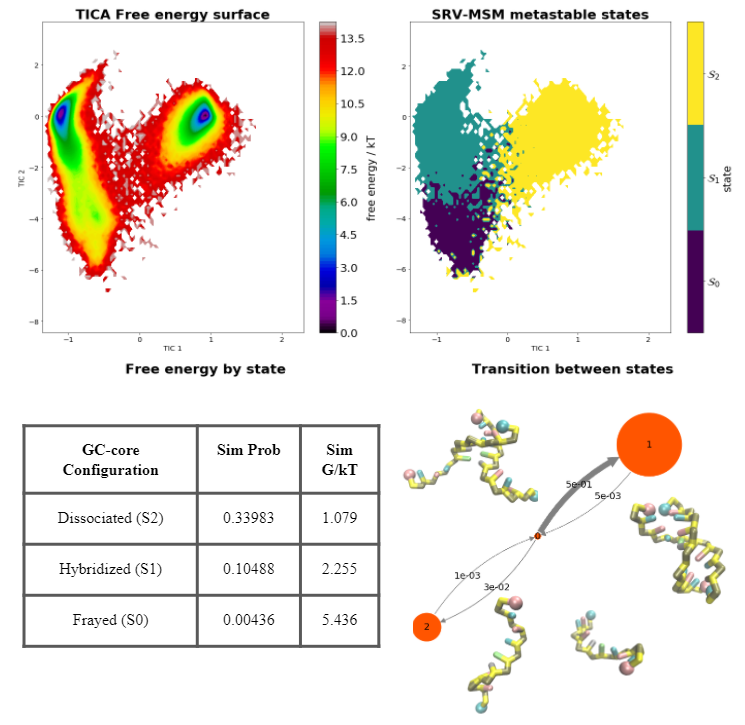
\includegraphics[width=\textwidth]{Figs/figs_0804/GC-core_thermo.PNG}
        \caption{Full MSM output for GC-core}
        \label{fig:GC-core_thermo}
	\end{center}
\end{figure}

\subsubsection{\label{sec:Results}Diffusion maps show ensemble of frayed states}

To further examine this 4bp-frayed state, we build diffusion maps using 10000 frames sampled from the macrostate \ref{fig:GC-core_dmaps}. This time, we set our distance metric to the same permutation-free coordinates we used to build the SRV-MSMs. Again, we were able to identify a combination of physical coordinates that closely correlated to the first two non-trivial diffusion modes. We found that a larger distance between the third and fourth A:T pairs increased the PCCA+ probability of inclusion into macrostate. This distance also correlated closely with the second diffusion map mode. Interestingly, we observed that the first non-trivial mode -- the feature that describes the most structural diversity in the system -- corresponds to difference in "overlap" distance between adjacent A or T bases and the GC core. In these conformations, one of the strands maintains some helical character while the other twist out of place, resulting in WC bonds being obstructed by the oligo backbone. These states represent another potential way in which the hybridization process (or helix reformation) can be kinetically frustrated. We observed this mode to be mostly symmetric, however there is slight tendency for the 3'T end to fray farther out of place relative to its 5'A counterpart. This might be another consequence of differential excluded volume radii in the 3spn2 force field.

\begin{figure}[ht!]
	\begin{center}
        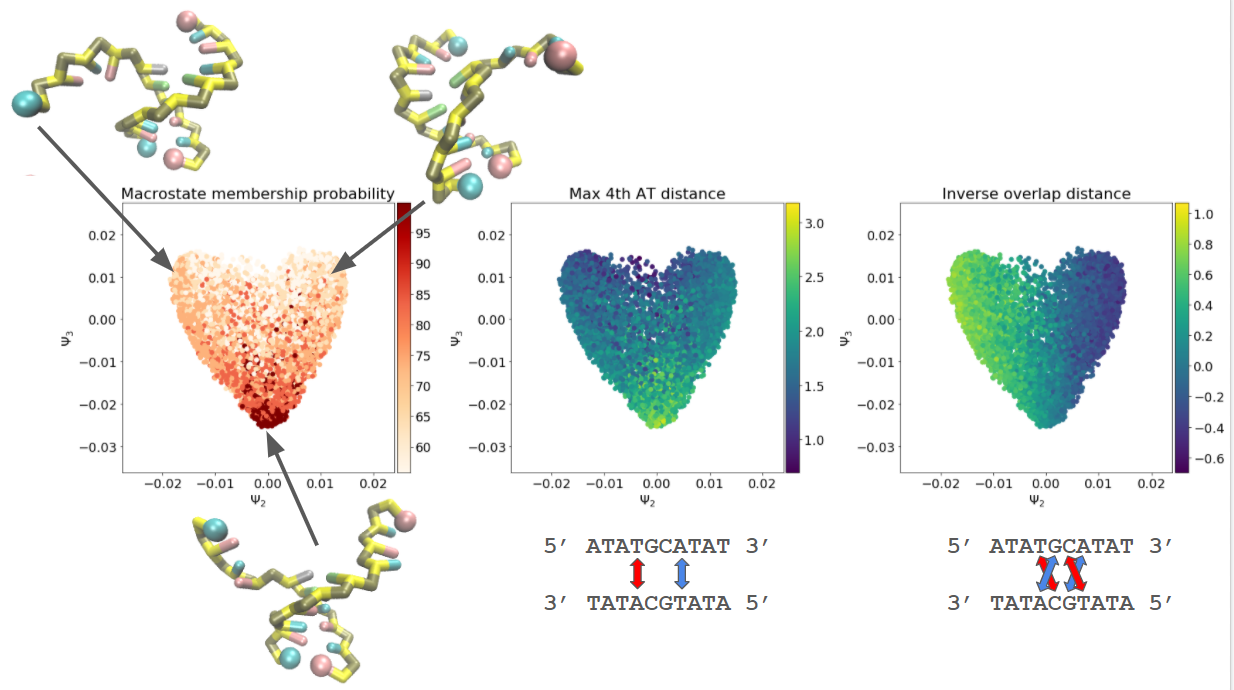
\includegraphics[width=\textwidth]{Figs/figs_0804/GC-core_dmaps.png}
        \caption{Plotting the first two non-trivial diffusion map eigenfunctions. Color maps show the probability that conformations are clustered into the frayed macrostate, maximum distance between 4th AT basepairs, and the the overlap between adjacent AT basepairs and the GC core.}
        \label{fig:GC-core_dmaps}
	\end{center}
\end{figure}

\subsubsection{\label{sec:Results}SRV correlations to physical coordinates?}

Having constructed and interpreted our SRV-MSM, we revisited our original SRV basis to analyze what physical correlations could be interpreted from the model. We found these GC-core modes to be of particular interest as they reveal the hierarchical nature of the dynamical encoding. We examined a collection of 1000-frame "trimmed" trajectories centered on both hybridization or dissociation events. For each trajectory, we compared the first three SRV coordinates with a corresponding collective variables with which they showed strong correlation. Two representative trajectories are shown in figure: (\ref{fig:GC-core_tracking_modes}). Complementary G:C pairs are the best indicators for a hybridization/dissociation event, and we see a sharp change in the first SRV mode (SRV1) as these bonds form or break. The second slow mode (SRV2) is most active when G:C pairs are bound but the adjacent AT pairs are not. There is a small signal for fraying at the outer base pairs, but the mode overwhelmingly learns about these neighboring A:T/G:C bonds. This behavior reflects the above-mentioned kinetic trap between core binding and the fully hybridized state. SRV3 is most active during dissociation, and seems to track closely with the average distance between all complementary base pairs. We attribute this to the SRV learning about the diffusive motions of the two body system. In addition to picking up on dissociation behavior, the third mode peaks when the oligos are close together but configured in such a way that is not amenable hybridization. These misaligned conformations include inverse contacts where 5'/5' and 3'/3' ends meet and looped conformations where one strand is folded in on itself and preventing satisfactory WC contacts. 

Despite the strong qualitative trends we observe between physical coordinates and leading SRV modes, we only find high Pearson correlations for SRV1. For the next two SRV modes, the sign of their correlation switches depending on whether the oligos are in the hybridized or dissociated state. This shows that these modes are providing support on top of the first mode -- which determines hybridization vs. dissociation -- and thus can display very different behaviors in either state. With respect to our SRV-MSM macroscates, we found that SRV2 was "turned on" in states 0 and 1 -- corresponding to the intact helix and frayed state, respectively -- and SRV3 was turned on in the dissociated state (S2). Accordingly, we recalculated Pearson correlations between each SRV mode and all distances in states where the modes are active. Figure \label{fig:GC-core_tracking_modes} shows the highest correlation between SRV2 and inner A:T pairs, weak correlation with outer A:T pairs, and an inverse correlation with 5'/5' and 3'/3' pairs which tend to approach each other during 4bp-fraying. We also observed a highly symmetric correlation between SRV3 and central base pairs distances, indicative of overall diffusive behavior. Taken together, these analyses reveal how the SRV learns and represents the dynamical space, leading to the MSM results we observe above.

\begin{figure}[ht!]
	\begin{center}
        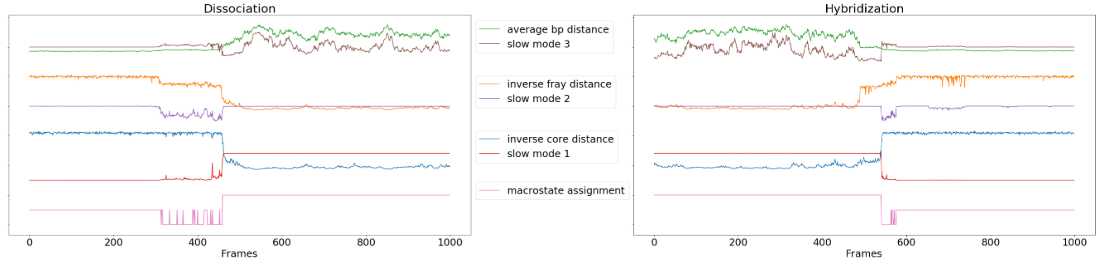
\includegraphics[width=\textwidth]{Figs/figs_0804/GC-core_tracking_modes.png}
        \caption{Show how SRV coordinates correspond to physical features over time and during sample dissociation and hybridization events. Should probably go to SI if we also include GC-core diffusion maps \textcolor{purple}{These single trajectory figures have proven useful for visualizing SRV dynamics, could be employed for GC-mix comparisons as well}}
        \label{fig:GC-core_tracking_modes}
	\end{center}
\end{figure}    


\subsubsection{\label{sec:Results}Comparison to Experiment}

When examining these same four sequences using T-jump IR and 2D IR spectroscopy, Sandstead et al. found that the GC-core had the highest deviation from two-state behavior during dissociation \citep{Sanstead2016}. As their lattice model did not consider previously mentioned shifted states, this intermediate state was defined by a high degree of fraying about the central core. While 1-2 base pair fraying was commonly observed for GC-mix and AT-all as well, lattice model predictions showed that GC-core had substantially more frayed base pairs \citep{Phys2019}. Variable T-jump measurements and Smoluchowski simulations on model 1D free energy landscapes showed that AT termini fraying was an effectively barrierless process characterized by rapid inter-conversion between all accessible frayed states \citep{Sanstead2018DirectDehybridization}. We see the same rapid fraying in simulation data -- which is too fast to be attributed to a converged SRV mode -- however we stipulate that this inter-conversion first relies on the formation of the the A:T bond nearest to the GC center. Our diffusion map analysis further shows how the ensemble of 4-bp frayed configurations impede helix formation. Although this process occurs much slower than single A:T base bonding and breaking, it may be difficult to experimentally discern from the overall hybridization process which contains both G:C and A:T character and occurs on a similar timescale.

%%%%%%%%%%%%%%%%%%%%%%%%%%%%%%%%%%%%%%%%%%%%%%%%%%%%%%%%%%%%%%%%

\subsection{\label{sec:Results}GC-mix}

The GC-mix sequence shows a similar implied timescale distribution to GC-core, however we no longer see a converged slow mode corresponding to multi-base fraying behavior. Instead, we observed two modes converge, corresponding to the association/dissociation dynamic and diffusive behavior while strands are dissociated. These correlate closely with the first and third GC-core SRV modes. Although we built our SRV-MSM using these two coordinates, we again were unable to form a stable third state along the second coordinate. As such, we designated this transitions as effectively two-state within the resolution of our model, however we do observe substantial fraying of the two AT termini in the simulation data. Although these frayed states may be too short-lived to resolve a distinct slow mode, this behavior shows qualitative agreement with experimental analysis of this sequence attributing fraying prior to dissociation as a deviation from all-or-nothing behavior \citep{Sanstead2016}.  While AT-termini fraying is surely a prerequisite to dissociation, we find these states to be so common and fleeting that very few progress to full dissociation. On the other hand, the 4bp-frayed state in GC-core had a substantial probability (~10\%) of fully dissociated rather reforming an intact helix. Furthermore, one or two base pair fraying does not fundamentally disrupt the helix in such a way that its re-formation is kinetically inhibited by the intermediate structures we present for GC-core.  

Given the lack of a repetitive AT interior (as in AT-all and GC-end) or consecutive AT exterior (as in GC-core), we expect more canonical dynamics from GC-mix. For this analysis, we looked at qualitative trends in our trajectory data, paying close attention to the distances between matching WC-pairs (\ref{fig:GC-mix_transitions}). During hybridization, we observe the formations of some key base pair contacts before the full duplex forms. Although it is statistically more likely for contact to form at the end of the duplex, we observe first contact at interior base pairs as well. This behavior is indicative of a nucleation-zippering mechanism as has been reported in previous studies \citep{Yin2011KineticsHybridization, Porschke1971CooperativeTransition}. We obverse dissociation events proceeded by two base pair fraying on one side of the duplex followed by more rapid dissociation of the central base pairs. There tends to be a short-lived state composed of 2-4 base pair contacts shortly before fully dissociation occurs. In contrast to the 4-bps frayed state we observe in GC-core, these conformations do not form a distinct free-energy minima in SRV or TICA space, nor do they tend to reform intact duplexes. As a whole, these dynamics are similar to previously reported "fraying-peeling" mechanism \citep{Wong2008TheSimulations, Perez2010Real-timeUnfolding, Zgarbova2014BaseRNA}. We observed similar fast dynamics and transition states in the other three sequences, however they are more difficult to discern as they occur in concert with the longer lasting metastable states discussed above.

\begin{figure}[ht!]
	\begin{center}
        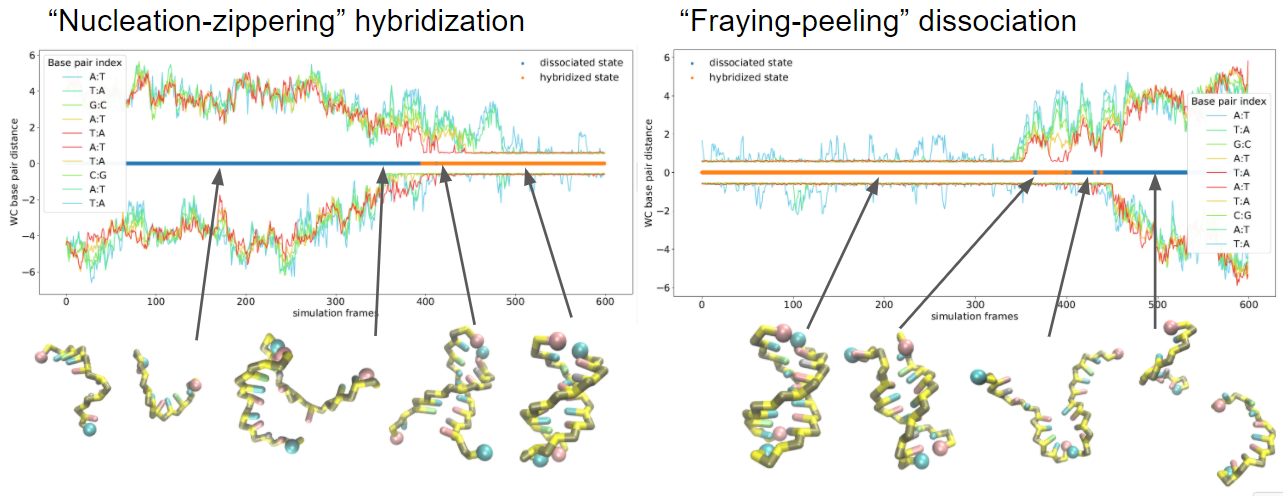
\includegraphics[width=\textwidth]{Figs/figs_0804/GC-mix_transitions.PNG}
        \caption{WC base pair distance and molecular renderings along two representative GC-mix hybridization and dissociation events.}
        \label{fig:GC-mix_transitions}
	\end{center}
\end{figure}

\subsubsection{\label{sec:Results}Temperature-dependent timescale comparisons}

Given differences in temperature and ensemble distributions between Tmelt simulations and T-jump experiments, we found it difficult to make direct timescales comparisons based on our equilibrium models alone. To supplement our analysis, we ran short simulations initialized in the hybridized state at a series of elevated temperatures for each sequence. We derived relaxation times for a "slow" dissociation response and "fast" fraying response at each temperature and compared these with experimental temperature-dependent relaxation fits for GC-end and GC-core \citep{Sanstead2018DirectDehybridization}. Although there was no experimental data for AT-all and GC-mix, we used our relaxation fits to predict how these might compare with the other sequences. We measure the slow dissociation response by fitting the distribution of times at which the core base pairs separate beyond a 2 nm cutoff. We find the inverse of these relaxation times -- the effective dissociation rate -- to increase exponentially with temperature, which is expected given the known thermodynamic influence on duplex stability. Furthermore, we see an acceleration of about one order of magnitude compared to experiment, although this factor is sensitive to the exact definition of melting temperature which can vary between simulation experiments. 

The fast response -- which Sanstead et. al attributed to single base pair fraying signatures -- was more difficult to compare given the limits our coarse-grained model. Numerous experimental and computational studies have shown that DNA and RNA fraying is a complex dynamical process with timescales that span 5 ps to several microseconds \citep{ Nonin1995TerminalFraying, Nikolova2012ProbingSimulations, Andreatta2006UltrafastHelix, Galindo-Murillo2015ConvergenceDGCACGAACGAACGAACGC}. Furthermore, all-atom simulations suggest that frayed ends can assume misaligned WC bonds, base-sugar hydrogen binding, and terminal stacked conformations\citep{PinamontiTheModels, Zgarbova2014BaseRNA}. Given that there is only one interaction site parameterized on each 3spn2 base, we would not expect to resolve this diverse collection of states and dynamics. Instead, we measure the fast fraying response by observing how long it takes for either duplex terminal end to split beyond a given cutoff. This approach assumes that fraying on the permutable top and bottom of the duplex are independent from each other, and that a base pair distance is a reliable approximation for the ensemble spectroscopy signal. This is a reasonable assumption given that the amplitude-weighted timescales should consist largely of terminal fraying events. For further comparison, we include fits over a range of cutoffs and repeat these calculations on the second and third interior base pairs.

For GC-core, each base pair and cutoff combination appears linear with temperature, indicating a barrierless and diffusion-driven process. As expected, the acceleration factor is also highly dependent on the choice of parameters, but, given that terminal fraying likely dominates the signal, we approximate that fraying dynamics are accelerated 100-300x relative to experiments. In contrast, GC-end is distinctly exponential, especially at base pairs closer to the core of the duplex. This behavior makes sense given the thermodynamic barrier to G:C fraying, but it also deviates the GC-end experimental linear fit. In addition to fraying, we notice that the rate of slithering increases at higher temperature. Moreover, the thermodynamic stability of these shifted conformations increases relative to that of intact duplex as temperature increases. For higher T-jumps, it is possible that a significant portion of the starting ensemble is in a shifted state (cite Ryan's work) and that the fast dynamics are increasingly influenced by slower "looping" G:C bonding that we observed in our diffusion map analysis above. It is less likely that shifting mechanisms would have their own distinct signals, given that these occur at far lower frequency than fraying or full-dissociation, but we believe that further experimental work is necessary to investigate this phenomenon.

The temperature-dependent analysis can also inform out interpretation of the 3spn2 model. Previous work has shows that kinetic association rates were accelerated by about 200x relative to experiment \citep{Hinckley2013AnHybridization}. This seems to be on the same order of magnitude as frayed acceleration, but dissociation is noticeably less accelerated when compared to experiment. It is not surprising that different dynamics might be accelerated at different rates, especially considering that 3spn2 was not parameterized based on any dynamical properties \citep{?}. 

%We also did not find available data on other acceleration studies using explicit ions.

\subsubsection{\label{sec:Results}Limitations} 

\begin{enumerate}
	\item Does not explicitly pick up on nucleation/zippering events. Because these are all unique sites (and zippering dynamics could vary at each site) it would be difficult to properly sample and interpret the unique corresponding mode. Furthermore these zippering dynamics occur significantly faster than slithering or GC-core fraying and cannot be captured via our save rate. 
	\item Coarse grain-models makes it difficult to compare timescales. Different degrees of freedom might have different accelerations.
	\item Limited by memory (number of frames) required to capture equilibrium trajectories at a save rate that enabled adequate resolution for the dynamics of interest.
	\item A smoother free energy surface minimizes the time spent in these intermediate states, and our featurization method is not sensitive to certain kinds of dynamics
	\item Sensitive to 3spn2 artefacts. Slithering may be overexpressed (and is in fact suppressed in \citep{Romano2013DNADependence}, but similar results have been shown in all-atom studies as well \citep{Xiao2019}. Base-pair mismatch interactions may be somewhat unphysical and alter state populations. Although we present slithering as a possible explanation for GC-end signal, there has been no conclusive evidence of these dynamics outside out all-atom and coarse-grained simulation studies. We hope that these data will present a 
	
\end{enumerate}


\subsection{\label{sec:Results}SI figs}


\begin{figure}[ht!]
	\begin{center}
        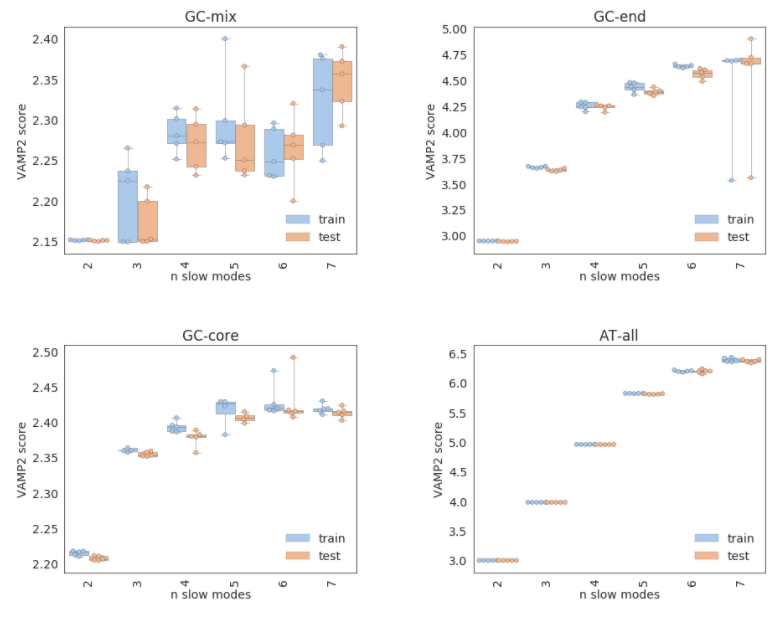
\includegraphics[width=\textwidth]{Figs/figs_0804/srv_crossval.png}
        \caption{5-fold cross validation procedure to select number of SRV coordinates. We look for both the converge of the VAMP-2 and consistent scores between folds to ensure that the model is not fitting on statistical noise. (probably will be SI, but could include AT-all cross-val in the walkthrough section)}
        \label{fig:srv_crossval}
	\end{center}
\end{figure}

\begin{figure}[ht!]
	\begin{center}
        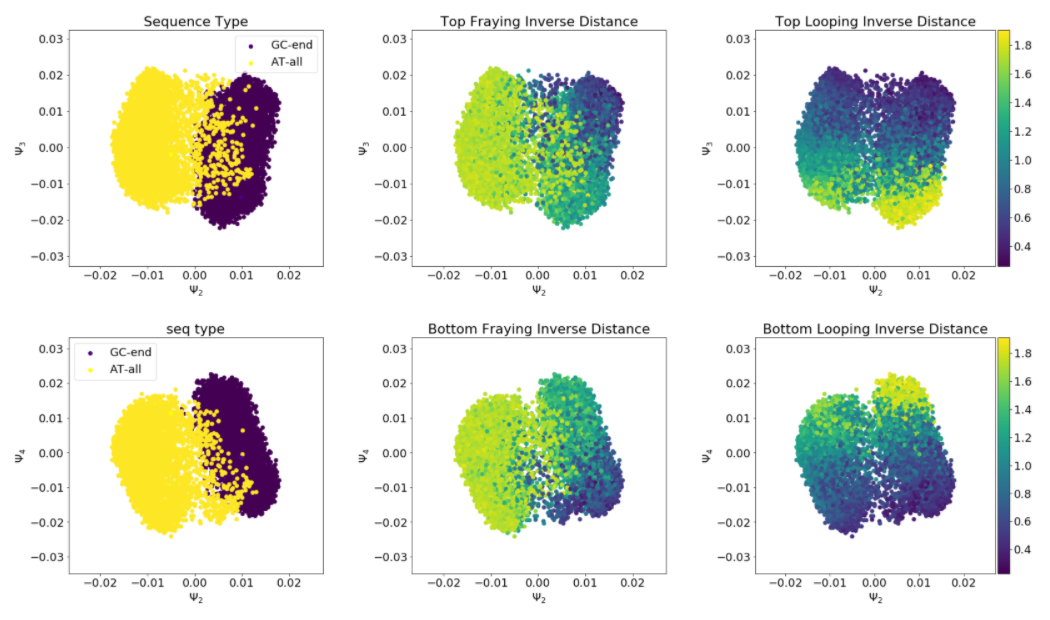
\includegraphics[width=\textwidth]{Figs/figs_0804/GC-end_dmaps_full.PNG}
        \caption{Full 5' diffusion maps including degenerate third diffusion map mode}
        \label{fig:GC-end_dmaps_full}
	\end{center}
\end{figure}

\begin{figure}[ht!]
	\begin{center}
        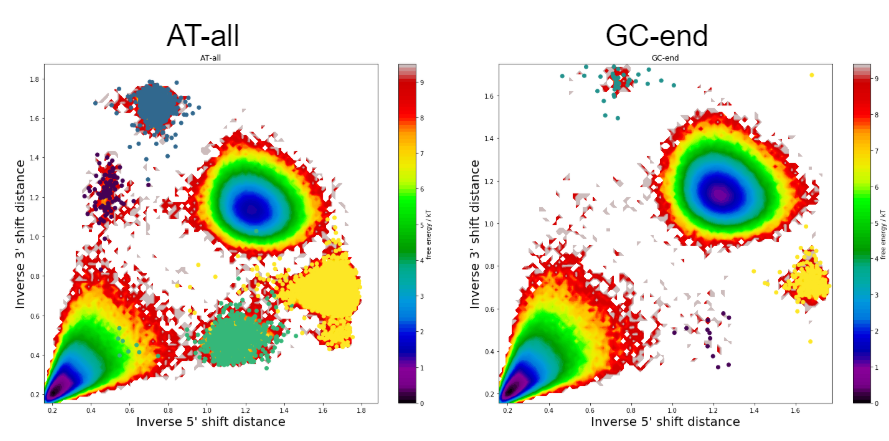
\includegraphics[width=\textwidth]{Figs/skeleton/shifting_distribution.PNG}
        \caption{Shows similarities between shifting modes and state memberships for AT-all and GC-ends (Not sure if this adds anything, if anything can grey out underlying free energy landscape and move this to the SI.}
        \label{fig:shifting_distributions}
	\end{center}
\end{figure}

\begin{figure}[ht!]
	\begin{center}
        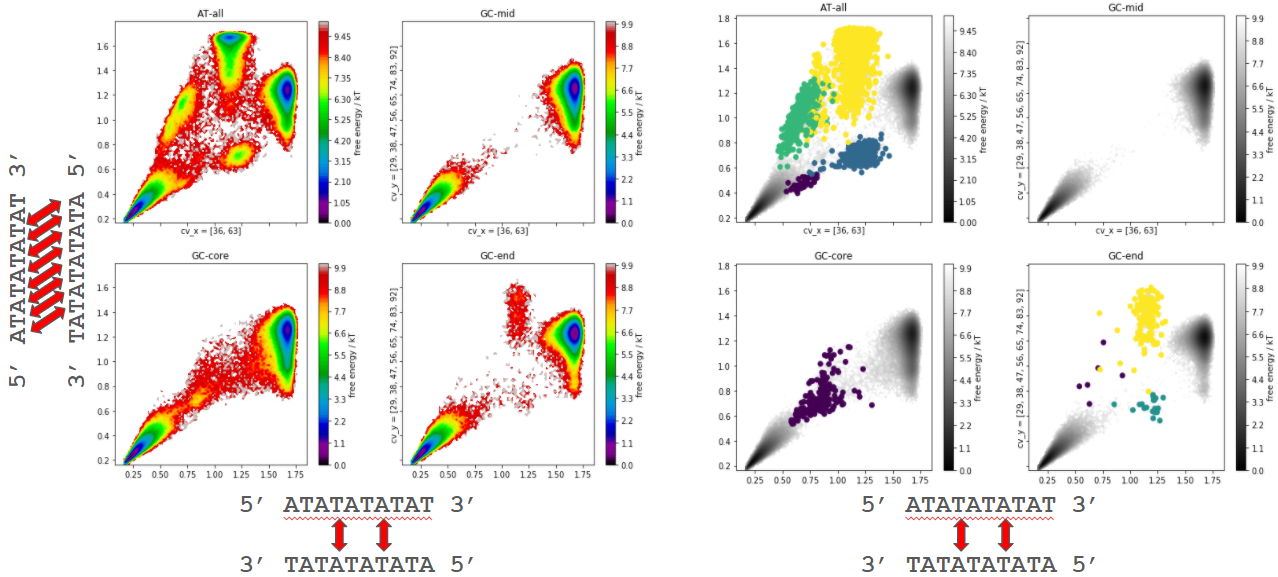
\includegraphics[width=\textwidth]{Figs/figs_0804/all_seq_physical_cvs_labels.PNG}
        \caption{All sequences and metastable macrostates plotted on frayed/shifted collective variable axes, Not sure how helpful these axes drawings are -- also need to switch x and y here.}
        \label{fig:all_seq_physical_cvs_labels}
	\end{center}
\end{figure}

\begin{figure}[ht!]
	\begin{center}
        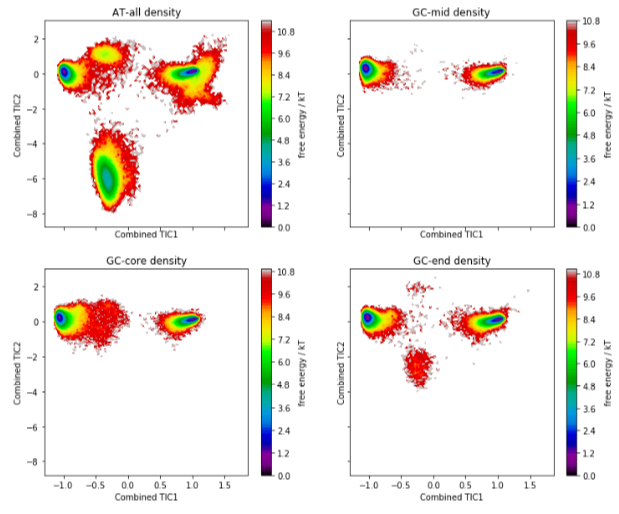
\includegraphics[width=\textwidth]{Figs/figs_0804/all_seq_tica_cvs.PNG}
        \caption{All sequences plotted on combined TICA axes. Might include in SI or not at all.}
        \label{fig:all_seq_tica_cvs}
	\end{center}
\end{figure}


\subsection{\label{sec:Results}Experimental comparisons across all sequences}

\subsubsection{\label{sec:Results}Thermodynamics of fraying align with lattice model}
Show similar distribution between lattice model and Tm data\citep{Phys2019}

\subsubsection{\label{sec:Results}Temperature-dependent correlations to slow and fast timescales}
Find approximate acceleration of model and find best physical comparison to fraying distances

\begin{comment}

Other ways to investigate GC-mix:
\begin{enumerate}

	\item Track GC-mid trajectories along transition region
	\item Discuss misaligned configurations here instead of in the GC-core section
\end{enumerate} 

Compare frayed thermo to Paul's lattice model predictions. 

\section{\label{sec:Discussion}Discussion}

\citep{Galindo-Murillo2015ConvergenceDGCACGAACGAACGAACGC}
Long simulations shows that terminal fraying does not converge on the picosecond timescale

\citep{Nonin1995TerminalFraying}
Most simulations suppress fraying by placing GC pairs at termini.

\citep{Andreatta2006UltrafastHelix}
- Base opening process is slower than 40 ns but faster than 1ms
- Open termini state shows new fraying mode of 5ps (I think shows free base motions)


\subsubsection{\label{sec:Results}Timescale comparison with experiment} 
SRV implied timescales pick up on an average time for the reversible transition A-->B-->A and thus describe the dwell time of kinetically relevant states discussed above. A more direct comparison to experiments can be made by examining the transition times of A-->B once the process has been initiated. In particular, we were interested in the fast and slow kinetic traces that were picked up by by Sandstead et al. To analyze the slow response -- which they attributed to overall strand dissociation -- we tried two methods. In the first, we used a variant of core sets where we defined "core regions" by PCCA+ probability of each microstate being clustered into a hybridized or dissociated macrostate \citep{PinamontiTheModels, (milestoning)}. We counted and averaged the number of frames between a 99 percent hybridized state and a 99 percent dissociated state, ensuring that the trajectory spend 10 consecutive frames in these cores before and after the transition, respectively. In the second method, we perform virtual relaxation experiments on each sequence-specific MSM (cite whoever built this method?). By assigning an initial probability distribution that favors microstates far from hybridized or dissociated regions, we can observe how this probability distribution shifts as the system relaxes to equilibrium. For each system there is fast response corresponding to the initial population finding its way to a more stable state, and a slow response showing the system reach global equilibrium. The fast response is providing information about the timescale of the transition itself and might be the best comparison. For GC-end and AT-all, a third signal is present representing equilibration from shifted states. There is some variation between sequences, but we find timescales of about 1-3 ns in simulation time. This is is about four orders of magnitude faster than the 13-32 (15-60 with updated data) us timescales reported by Sandstead et al.

The fast response Sanstead et. al -- attributed to single base pair fraying signatures -- was more difficult to compare given the limits our coarse-grained model. Numerous experimental and computational studies have shown that DNA and RNA fraying is a complex dynamical process with timescales that span 5 ps to several microseconds \citep{ Nonin1995TerminalFraying, Nikolova2012ProbingSimulations, Andreatta2006UltrafastHelix, Galindo-Murillo2015ConvergenceDGCACGAACGAACGAACGC}. Furthermore, all-atom simulations suggest that frayed ends can assume misaligned WC bonds, base-sugar hydrogen binding, and terminal stacked conformations\citep{PinamontiTheModels, Zgarbova2014BaseRNA}. Given that there is only one interaction site parameterized on each 3spn2 , we would not expect to resolve this diverse collection of states and dynamics. To obtain a rough metric for terminal base fraying, we ran shorter simulations with a more frequent save rate and calculated an averaged transit time from the closed to open state (SI). We observed substantial variability in fraying behavior, but overall we found transit times to be within 5-20 ps in simulation time. If we compare these to fast response timescales of Sanstead et al., we find that these rates are again accelerated by about four orders of magnitude.

Previous studies with 3spn2 showed a 200x acceleration when looking at kinetic association rates alone \citep{Hinckley2013AnHybridization}. When we examine higher order processes, such at dissociation transit time and single-base fraying, we observed a more substantial acceleration of nearly four order of magnitude. This is not surprising given that a smoothened free energy landscape would have a more substantial effect on higher order dynamics than the diffusion-limited pathways that determine association.

\end{comment}


\subsubsection{\label{sec:Results}Code to provide on GitHub} 
\begin{enumerate}
    \item{Cross val data}
    \item lammps run script and each sequence input files
    \item Featurization with mdtraj (reindexing and sparse saving)
    \item Dmaps for GC-core and GC-end
    \item timescales comparison
    \item MSM construction
\end{enumerate}

\section{\label{sec:conc}Conclusion}
\subsection{\label{sec:Results}Will look a lot like the last paragraph of the intro / the abstract}

\begin{comment}

%%%%%% Other MSM and timescales approaches  %%%%%%%%%%%

McGibbon, R. T., & Pande, V. S. (2015). Variational cross-validation of slow dynamical modes in molecular kinetics : Importance of not generating too many microstates and employting cross-validation to avoid artificially high scores or artificially slow dynamics. Both of these lead to models fitting statistical noise which is the root of boosted scores.

Pinamonti, G., Paul, F., Rodriguez, A., & Bussi, G. (n.d.). analyzed with core-set Markov state models, 43: Good ideas on core-based clustering. Assigning microstates based on physical characteristics is interesting but didn't seem to work for me in practice (could try doing this based on sim.log data with number of base pairs bound or some energy metric). Lot's of notes on this paper regarding comparisons to timescales. Good notes on higher resolution fraying interactions that we likely can't resolve.

Sua, E., Adelman, J. L., & Zuckerman, D. M. (2016). Accurate Estimation of Protein Folding and Unfolding Times : Beyond Markov State Models, 1. https://doi.org/10.1021/acs.jctc.6b00339:
More accurate ways to adapt MFPT into a rate

Refs for DNA fraying:
\citep{Hagan2003AtomisticDNA} Atomistic simulations for biosensign app (can include in intro). Use TPS to focus on kinetic pathway by which singl base pair bind/unbind. Focus on end base of 3-bp oligomer in explicit solvent. Finds order parameters tracking base pair binding as well as intra-strand stacking. (energy and distance for each). 

\citep{Wong2008TheSimulations} Three step melting process: untwisting most important,

6K.-Y. Wong and B. M. Pettitt, “The pathway of oligomeric DNA melting investigated by molecular dynamics simulations,” Biophys. J. 95, 5618– 5626 (2008).
37A. Perez and M. Orozco, “Real-time atomistic description of DNA unfold- ing,” Angew. Chem. 49, 4805–4808 (2010).
38M. F. Hagan, A. R. Dinner, D. Chandler, and A. K. Chakraborty, “Atomistic understanding of kinetic pathways for single base-pair binding and unbinding

\end{comment}


\clearpage
\newpage

%\bibliography{references}
\bibliography{refs_mendeley2}

%%%%%%%%%%%%%%%%%%%%%%%%%%%%%%%%%%%%%%%%%%%%%%%%%%%%%%%%%%%%%%%%%%%%%
%% The "tocentry" environment can be used to create an entry for the
%% graphical table of contents.
%%%%%%%%%%%%%%%%%%%%%%%%%%%%%%%%%%%%%%%%%%%%%%%%%%%%%%%%%%%%%%%%%%%%%

\clearpage


\end{document}
